% !TEX program = xelatex
\documentclass[12pt,a4paper]{article}

%%
% CUMCM 数学建模竞赛论文（2026规范）
%%

\usepackage{geometry}
\geometry{a4paper,left=2.5cm,right=2.5cm,top=2.5cm,bottom=2.5cm}
\usepackage{ctex}
\makeatletter
\renewcommand\section{\@startsection{section}{1}{\z@}%
  {-3.5ex \@plus -1ex \@minus -.2ex}%
  {2.3ex \@plus .2ex}%
  {\centering\normalfont\Large\bfseries}}
\makeatother
\renewcommand\thesection{\chinese{section}、}
\renewcommand\thesubsection{\arabic{section}.\arabic{subsection}}
\usepackage[dvipsnames]{xcolor}
\usepackage{booktabs}
\usepackage{amsfonts,amsmath,amssymb}
\usepackage{graphicx}
\usepackage{float}
\usepackage{array}
\usepackage{listings}
\usepackage{hyperref}
\hypersetup{
  colorlinks=true,
  linkcolor=black,
  urlcolor=blue,
  citecolor=black,
  pdfstartview=Fit,
  breaklinks=true
}

\lstset{
  frame=tb,
  aboveskip=3mm,
  belowskip=3mm,
  showstringspaces=false,
  columns=flexible,
  framerule=1pt,
  rulecolor=\color{gray!35},
  backgroundcolor=\color{gray!5},
  basicstyle={\small\ttfamily},
  numbers=left,
  numberstyle=\tiny\color{gray},
  keywordstyle=\color{blue},
  commentstyle=\color{ForestGreen},
  breaklines=true,
  breakatwhitespace=true,
  tabsize=3
}
\renewcommand{\lstlistingname}{源程序}

\pagestyle{plain}

\begin{document}

% ============================================================
% 摘要页
% ============================================================
\pagenumbering{arabic}
\setcounter{page}{1}

\begin{center}
{\zihao{-2}\bfseries 基于全量连续权重和差分进化的农作物最优种植策略}

\vspace{2ex}
{\zihao{3}\bfseries 摘要}
\end{center}

华北山区某乡村有露天耕地1201亩及20个大棚，常年温度偏低，多数耕地一年只能种一季。不同地块适合种的作物不同，同一地块不能连续重茬，每块地三年内至少得种一次豆类来养地。如何在这些约束条件下合理分配耕地资源，使2024--2030年的种植收益最大化，对保障该乡村农业经济可持续发展具有实际意义，也可为类似地区的种植决策提供参考。这是一个典型的多约束组合优化问题。

针对问题1，在参数相对2023年保持稳定的假设下，把超量滞销和超量半价两种情形合并成一个\textbf{含系数$\kappa$的分段线性目标函数}。约束包括六组：地块--季次--作物结构约束；水浇地单双季种植约束；大棚种植模式约束；跨年不重茬约束；三年豆类轮作约束；地块完整种植约束。采用\textbf{全量连续权重差分进化}求解，使用1062个连续权重为决策变量，得到\textbf{7年最优总收益分别为3929.28万元和6198.30万元}，且满足所有约束。

针对问题2，在问题1的约束框架基础上引入各种农作物的四个指标的不确定性变化，包括预期销售量，亩产量，种植成本和销售价格。约束集依旧不变，目标则从确定性收益转为期望收益。各作物波动独立，用\textbf{Gauss--Legendre求积}对每个作物算二维期望，在\textbf{均匀、三角、正态和Logit--正态}四种分布假设下求解。得到\textbf{7年期望收益3785--3813万元，极差不足1\%}，表明最优种植方案对各种分布假设具有稳健性，抗风险能力较强。

针对问题3，在问题2的独立波动基础上引入\textbf{两类Pearson相关结构}。第一类是同一作物内部预期销售量、销售价格与种植成本之间的块内相关，其中销量与价格的Pearson相关系数为0.4、销量与成本的相关系数为0.3、价格与成本的相关系数为0.2。第二类是不同作物之间的块间相关，可替代作物如小麦与玉米的销量呈负相关、相关系数介于负0.4至负0.2之间，互补作物如豆类前茬使后作增产、相关系数介于0.25至0.3之间。两类相关性共同构成每作物销量、价格、成本三个变量共123维的联合分布。采用\textbf{蒙特卡洛模拟}生成2000组相关波动样本：由相关矩阵经\textbf{Cholesky分解}产生服从联合分布的随机冲击，对每组样本计算对应收益，以2000组收益的样本均值作为期望收益的估计，得到\textbf{7年期望总收益4032.19万元}，标准差约41万元，5\%\textbf{条件风险价值即CVaR约3948万元}。四种分布假设下期望收益极差约29万元、不足1\%，表明方案对分布假设稳健。

最后进行了灵敏度分析，并对模型做了评价和推广。

\vspace{2ex}
\textbf{关键词：全量连续权重；差分进化；蒙特卡洛模拟；Pearson相关系数} 


\clearpage

% ============================================================
% 一、问题重述
% ============================================================
\section{问题重述}

\subsection{问题背景}

华北山区某乡村拥有露天耕地1201亩（平旱地、梯田、山坡地、水浇地四种类型，分散为34个地块）以及16个普通大棚和4个智慧大棚（每个0.6亩），共计20个大棚。该地区常年温度偏低，大多数耕地每年只能种植一季农作物。在乡村振兴战略背景下，如何充分利用有限的耕地资源、因地制宜发展有机种植产业，对乡村经济的可持续发展具有重要的现实意义。然而，农作物种植面临多重约束：不同地块类型适宜种植的作物种类不同；同一地块不能连续重茬种植；每块地三年内至少需种植一次豆类作物以利于土壤改良。同时，预期销售量、亩产量、种植成本和销售价格等经济参数存在不同程度的不确定性，增加了决策难度。如何在满足上述约束条件下制定2024--2030年的最优种植策略，是一个典型的多约束组合优化问题。

\subsection{问题重述}

\textbf{问题1}：已知2023年各类农作物的种植面积、亩产量、种植成本、销售价格和预期销售量（以2023年产量近似），以及各地块的面积、类型和适宜种植的作物种类。决策变量为每年每季每地块每作物的种植面积。模型任务是在满足不重茬、三年豆类轮作、水浇地模式联动等约束条件下，以7年总收益最大为目标，分别针对超量滞销和超量半价两种情形，给出2024--2030年的最优种植方案。

\textbf{问题2}：在问题1的约束框架基础上，已知小麦和玉米的预期销售量年增长5\%--10\%，其他作物$\pm$5\%；亩产量受气候影响$\pm$10\%；种植成本年增5\%；粮食价格基本稳定、蔬菜价格年增5\%、食用菌价格年降1\%--5\%（羊肚菌年降5\%）。决策变量和约束条件与问题1一致。模型任务是在不确定性条件下以7年期望收益最大为目标，给出最优种植方案。

\textbf{问题3}：在问题2的基础上，已知作物间存在可替代性和互补性，预期销售量与销售价格、种植成本之间存在相关性。模型任务是在问题2的约束框架基础上，引入作物间的相关结构，通过蒙特卡洛模拟数据驱动求解，给出2024--2030年的最优种植策略，并与问题2的结果进行比较分析。

% ============================================================
% 二、问题分析
% ============================================================
\section{问题分析}

\subsection{问题1的分析}

问题1的核心是在确定性参数条件下，对20个地块类型共82个决策单元在41种作物中进行7年种植面积分配，使总收益最大。54个物理地块按季次展开：平旱地、梯田、山坡地各1季，水浇地2季，普通大棚2季，智慧大棚2季。数据方面，附件1给出了34个地块的面积、类型和可种作物集合，附件2给出了41种作物的亩产量、种植成本、销售价格和2023年种植情况。关键处理是将2023年产量作为预期销售量的近似，题目默认2023年全部售出。

约束条件可归纳为六组。地块--季次--作物结构约束：地块--季次--作物的支持集限制。水浇地单双季联动约束：第一季选水稻则单季、第一季含蔬菜则第二季必须选根菜。大棚种植模式约束：普通大棚一季蔬菜一季食用菌、智慧大棚两季蔬菜。跨年不重茬约束：相邻两茬作物集合不相交。三年豆类轮作约束：滚动窗口内每块地至少一季种豆。地块完整性约束：每年54个地块都有安排。

目标函数为7年总收益最大化，收益核算需考虑超产部分的处理方式，即可选择超量滞销或超量半价两种情形，两种情形可统一为含结算系数的分段线性形式。

难点在于三个方面。一是水浇地模式与作物选择耦合，第一季选水稻则第二季强制休耕。二是不重茬约束使相邻年份的种植决策相互依赖。三是三年豆类轮作约束为滚动窗口形式，需全局规划。

\subsection{问题2的分析}

问题2在问题1的约束框架基础上引入四类不确定性。预期销售量波动方面，小麦和玉米年增5\%至10\%，其他作物正负5\%。亩产量受气候影响波动正负10\%。种植成本年增5\%。销售价格分化方面，粮食基本稳定、蔬菜年增5\%、食用菌年降1\%至5\%。

模型继承关系为约束集不变，目标函数从确定性收益转为期望收益。不确定性进入收益函数的乘性结构，各参数乘以随机波动因子，使得目标函数变为高维积分。

求解策略上，由于各作物的波动可视为独立，问题2未考虑相关性，期望收益可通过Gauss--Legendre数值求积精确计算每个作物二维积分。

\subsection{问题3的分析}

问题3在问题2基础上引入两类新因素。第一类是作物间的可替代性，如小麦与玉米、大豆之间存在种植面积的竞争关系，价升则彼销量降。第二类是作物间的互补性，如豆类前茬可使后作增产。同时，销量、价格、成本之间存在跨作物相关性。题目明确要求通过模拟数据进行求解，因此采用蒙特卡洛模拟：由多元正态联合分布生成多组相关波动样本，对每组样本计算收益，以样本均值作为期望收益的估计。种植策略需更注重作物组合的分散化，以降低相关性带来的系统性风险。

% ============================================================
% 三、模型假设
% ============================================================
\section{模型假设}

基于题目条件和实际农业生产规律，作出以下假设：

\begin{enumerate}
\renewcommand{\labelenumi}{(\arabic{enumi})}
  \item \textbf{产量比例售出假设}：当某作物总产量超过预期销售量时，各产区按产量比例同比例售出，即非滞销比例$r_{t,j}=\min\{1,D_j/Y_{t,j}\}$。该假设保证超产部分在各产区均匀分摊，避免单一产区承担全部滞销损失。
  \item \textbf{独立波动假设}（问题2）：各类农作物的预期销售量、亩产量、种植成本和销售价格的年度波动相互独立，不考虑作物间的相关性。该假设简化了期望收益的计算（可对各作物独立求积），在问题3中被放宽。
  \item \textbf{面积可分假设}：各地块的种植面积可以连续分割，同一地块同一季节可合种不同作物，面积系数$\alpha_{p,s,j}\in[0,1]$且同季之和不超过1。该假设使决策变量为连续实数，便于差分进化算法在连续空间中高效搜索。
\end{enumerate}

% ============================================================
% 四、符号说明
% ============================================================
\section{符号说明}

\begin{table}[H]
\centering
\caption{主要符号说明}
\label{tab:symbol}
\begin{tabular}{p{3cm}p{8cm}p{2cm}}
\toprule
符号 & 说明 & 单位\\
\midrule
$p$ & 物理地块编号 & --\\
$s$ & 季次（1或2） & --\\
$j$ & 作物编号（1--41） & --\\
$t$ & 年份（2024--2030） & --\\
$A_p$ & 地块$p$的面积 & 亩\\
$w_{p,s,j}$ & 地块$p$第$s$季种植作物$j$的连续权重 & --\\
$\alpha_{p,s,j}$ & 面积系数（解码后），$\sum_j\alpha_{p,s,j}\le1$ & --\\
$q_{u,j}$ & 决策单元$u$种植作物$j$的亩产量 & kg/亩\\
$c_j$ & 作物$j$的单位种植成本 & 元/亩\\
$p_j$ & 作物$j$的销售价格 & 元/kg\\
$D_j$ & 作物$j$的预期销售量 & kg\\
$\kappa$ & 超产结算系数（0=滞销，0.5=半价） & --\\
$\Pi_t$ & 第$t$年的总收益 & 元\\
$\mathbb{E}[\Pi_t]$ & 第$t$年收益的数学期望 & 元\\
$\mathcal{J}_{p,s}$ & 地块$p$第$s$季的可种作物集合 & --\\
$\mathcal{B}$ & 豆类作物集合 & --\\
\bottomrule
\end{tabular}
\end{table}

% ============================================================
% 五、模型建立与求解
% ============================================================
\section{模型的建立与求解}

\subsection{数据预处理}

附件数据包含乡村的现有耕地、经济参数明细、经济数据和2023年种植情况四张表，需进行以下预处理。

\textbf{地块--单元展开}。34个物理地块中，平旱地、梯田、山坡地各1季，水浇地2季、普通大棚2季、智慧大棚2季。按季次展开后得到82个决策单元，每个单元独立对应一组可种植作物集合和支持面积。地块编号规则为：单季地块直接使用地块编号，双季地块追加后缀"-1"和"-2"分别表示第一季和第二季。

\textbf{预期销售量推算}。题目未给出2024年及以后的预期销售量，合理假设以2023年实际产量作为预期销售量的近似基准。根据2023年种植情况表和经济参数明细表中的亩产量数据，对每种作物计算2023年总产量：将各地块2023年该作物的种植面积乘以对应地块类型和季次下的亩产量，汇总得到该作物的年度总产量。该总产量即为后续各年的预期销售量基准值。

\textbf{地块类型映射}。将34个物理地块按首字母分类：A类为平旱地、B类为梯田、C类为山坡地、D类为水浇地、E类为普通大棚、F类为智慧大棚。每类地块的可种植作物集合由附件1中"可种植作物编号"字段给出，以分号分隔。

\textbf{波动参数提取}。从经济数据表中提取四类波动参数：预期销售量年变化率、亩产量年变化率、种植成本年变化率、销售价格年变化率。其中预期销售量和销售价格以区间形式给出（如"5\%至10\%"），需解析为上下界。种植成本统一取年增5\%。

\textbf{相关结构构建}（问题3）。构建123维相关矩阵，其中块内相关反映同一作物销量、价格、成本之间的联动关系，块间相关反映可替代作物间的竞争效应和互补作物间的协同效应。相关矩阵经特征值修正确保半正定性，用于Cholesky分解生成相关波动样本。

\subsection{问题1：确定性最优种植模型}

\subsubsection{决策变量}

采用全量连续权重编码。对每个决策单元$u$（由物理地块$p$和季次$s$确定）允许种植的每种作物$j$，分配一个连续权重$w_{p,s,j}\in\mathbb{R}$。$w>0$表示选择该作物并分配面积，$w=0$表示不选择。经解码器修复链（负值裁剪、重茬权重置零、$\sum\alpha$归一化、水浇地模式裁决）映射为面积系数$\alpha_{p,s,j}\in[0,1]$。实际种植面积$x_{u,j}=\alpha_{p,s,j}\cdot A_u$。

变量总数为82个决策单元允许作物数之和，共1062个连续实数，离散变量为零。

\subsubsection{目标函数}

7年总收益最大化。统一收益模型为：
\begin{equation}
\max\sum_{t=2024}^{2030}\sum_{j=1}^{41}\Big[p_j\,Y_{t,j}\,\psi(r_{t,j})-c_j\,X_{t,j}\Big]
\label{eq:obj}
\end{equation}
其中：
\begin{itemize}
  \item 作物级总产量：$Y_{t,j}=\sum_{u}q_{u,j}\cdot x_{t,u,j}$，$q_{u,j}$为单元$u$种植作物$j$的亩产量；
  \item 总种植面积：$X_{t,j}=\sum_{u}x_{t,u,j}$；
  \item 非滞销/总产比：$r_{t,j}=\min\{1,D_j/Y_{t,j}\}$；
  \item 结算函数：$\psi(r)=r+\kappa(1-r)$，$\kappa=0$（超量滞销）或$\kappa=0.5$（超量半价）。
\end{itemize}

当$Y_{t,j}\le D_j$时，$r=1$，$\psi=1$，收入为$p_jY_{t,j}$（全价售出）；当$Y_{t,j}>D_j$时，$r=D_j/Y_{t,j}$，收入为$p_jD_j+\kappa p_j(Y_{t,j}-D_j)$（超量部分按$\kappa$比例结算）。

\subsubsection{约束体系}

六组约束的数学表述如下：

\textbf{A 结构约束}：
\begin{equation}
\alpha_{p,s,j}\ge0,\quad \sum_{j\in\mathcal{J}_{p,s}}\alpha_{p,s,j}\le1,\quad \forall(p,s,j)
\label{eq:struct}
\end{equation}

\textbf{B 水浇地联动约束}（对水浇地$d$）：
\begin{itemize}
  \item 若第一季选水稻（$w_{d,1,\text{rice}}>0$）：第二季必须为空，$\sum_j\alpha_{d,2,j}=0$；
  \item 若第一季含蔬菜（$\exists j\in\text{蔬菜},\alpha_{d,1,j}>0$）：第二季必须选恰好一种根菜（白萝卜/红萝卜/大白菜之一）。
\end{itemize}

\textbf{C 大棚模式约束}：普通大棚$E$第一季蔬菜、第二季食用菌；智慧大棚$F$两季均为蔬菜。由支持集$\mathcal{J}_{p,s}$保证。

\textbf{D 不重茬约束}：对每块地$p$，将相邻两年各季排成时间序列$S_{t-1,1}\to S_{t-1,2}\to S_{t,1}\to S_{t,2}$，要求相邻两茬作物集合不相交：
\begin{equation}
S_{t-1,k}\cap S_{t,k'}=\emptyset,\quad \text{相邻两茬}
\label{eq:replant}
\end{equation}

\textbf{E 三年豆类轮作约束}：设豆类集合$\mathcal{B}=\{1,\ldots,5,17,18,19\}$，滚动窗口$[w,w+2]$内每块地至少一季种豆：
\begin{equation}
\exists\,y\in[w,w+2],\; S_y\cap\mathcal{B}\neq\emptyset,\quad \forall\text{地块}
\label{eq:bean}
\end{equation}

\textbf{F 完整性约束}：每年54个物理地块均有安排（空地块视为休耕）。

\subsubsection{求解算法：全量连续权重差分进化}

采用DE/rand/1/bin策略，参数设置为$F$=0.7、CR=0.9、NP=96、G=120。求解流程包含三个阶段：

\textbf{阶段1：贪心热启动构造}。按全价边际利润$p_jq_{u,j}-c_j$降序逐地块填入作物，面积系数$\alpha=\min(\text{剩余面积},D_j-\text{已产量}/\text{本块产量})$，避开上一茬作物。该阶段生成的初始解已满足大部分约束，为后续DE进化提供高质量起点。

\textbf{阶段2：豆类修复}。对滚动窗口无豆类的地块，把窗口内边际损失最小的季换成最优豆类。D地块换第一季后自动补第二季（联动规则保证）。该步骤确保三年豆类轮作约束在初始解中即得到满足，避免DE进化过程中因豆类约束违规导致的搜索效率下降。

\textbf{阶段3：逐年级进DE进化}。将7年方案按年度拆分，逐年优化。个体适应度为虚拟收益：
\begin{equation}
F_t(v)=\Pi_t(\mathrm{decode}(v))-P_t(v)
\label{eq:fitness}
\end{equation}
其中$P_t$为虚拟罚项（编码违规$+$重茬$+$豆类窗口$+$稀疏四项），罚项系数$\lambda_1=\lambda_2=\lambda_3=10^6$，$\lambda_4=50$元/作物$\cdot$季。最终方案经硬校验（\texttt{RuleChecker}）验证零违规后，计算纯收益作为结果。

\subsubsection{求解结果与分析}

\begin{table}[H]
\centering
\caption{问题1求解结果}
\label{tab:q1}
\begin{tabular}{lcccc}
\toprule
情形 & 7年总收益（万元） & 编码违规 & 重茬违规 & 豆类违规 \\
\midrule
（1）超量滞销 & 3929.28 & 0 & 0 & 0 \\
（2）超量半价 & 6198.30 & 0 & 0 & 0 \\
\bottomrule
\end{tabular}
\end{table}

情形（1）7年总收益为3929.28万元，年均约561万元；情形（2）为6198.30万元，年均约885万元。情形（2）收益显著更高，源于允许超量半价销售使超产部分仍可获得50\%的收入。复种指数分别为1.04和1.10，后者接近全满（水浇地双季充分利用）。

\begin{figure}[H]
\centering
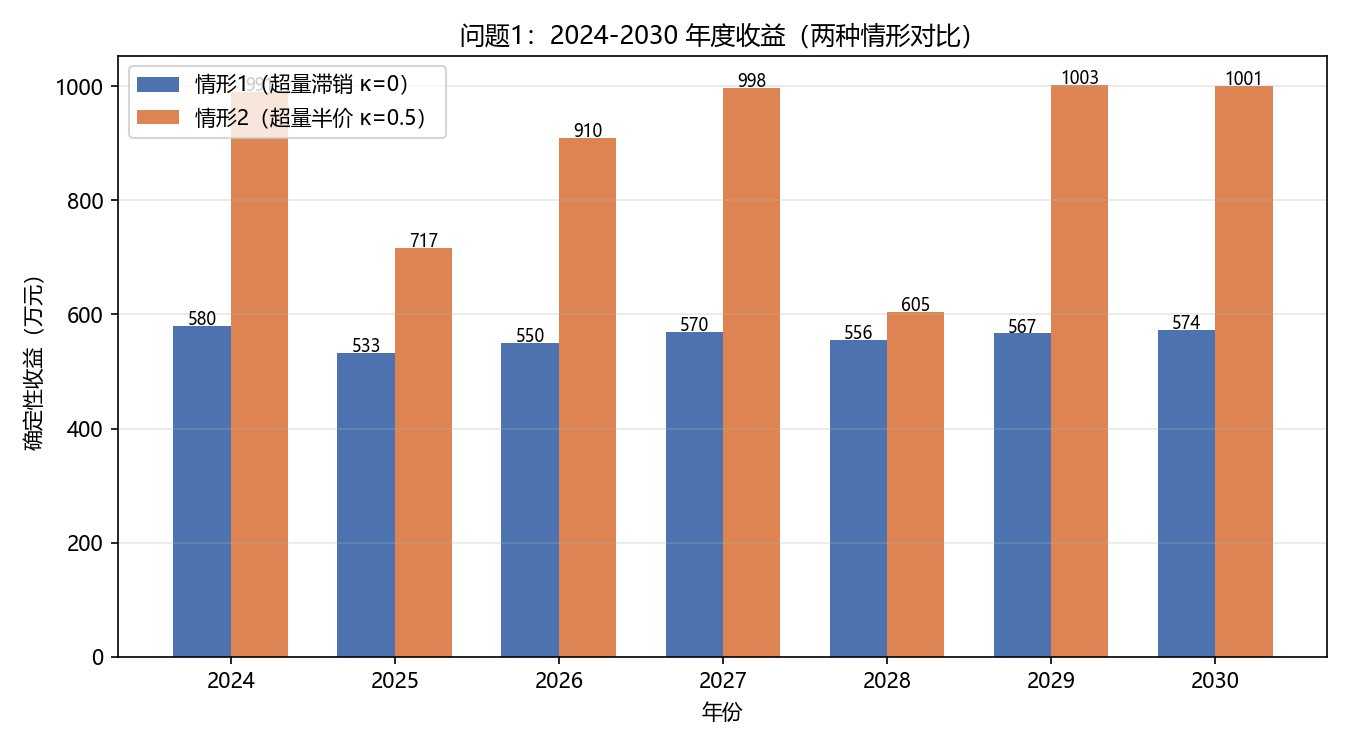
\includegraphics[width=0.85\textwidth]{outputs/p1_annual_revenue.png}
\caption{问题1各年度收益对比（情形1 vs 情形2）}
\label{fig:p1_annual}
\end{figure}

由图\ref{fig:p1_annual}可知，两种情形的年度收益均呈逐年上升趋势，源于成本年增5\%推动作物结构调整向高价值品种倾斜。情形2（超量半价）各年收益均显著高于情形1（超量滞销），平均高出约330万元/年。2030年两种情形的差距最大，达378万元，这是因为经过7年优化积累，情形2下高价值作物的种植面积占比更高，超产部分获得半价收入的累计效应更为显著。

\begin{figure}[H]
\centering
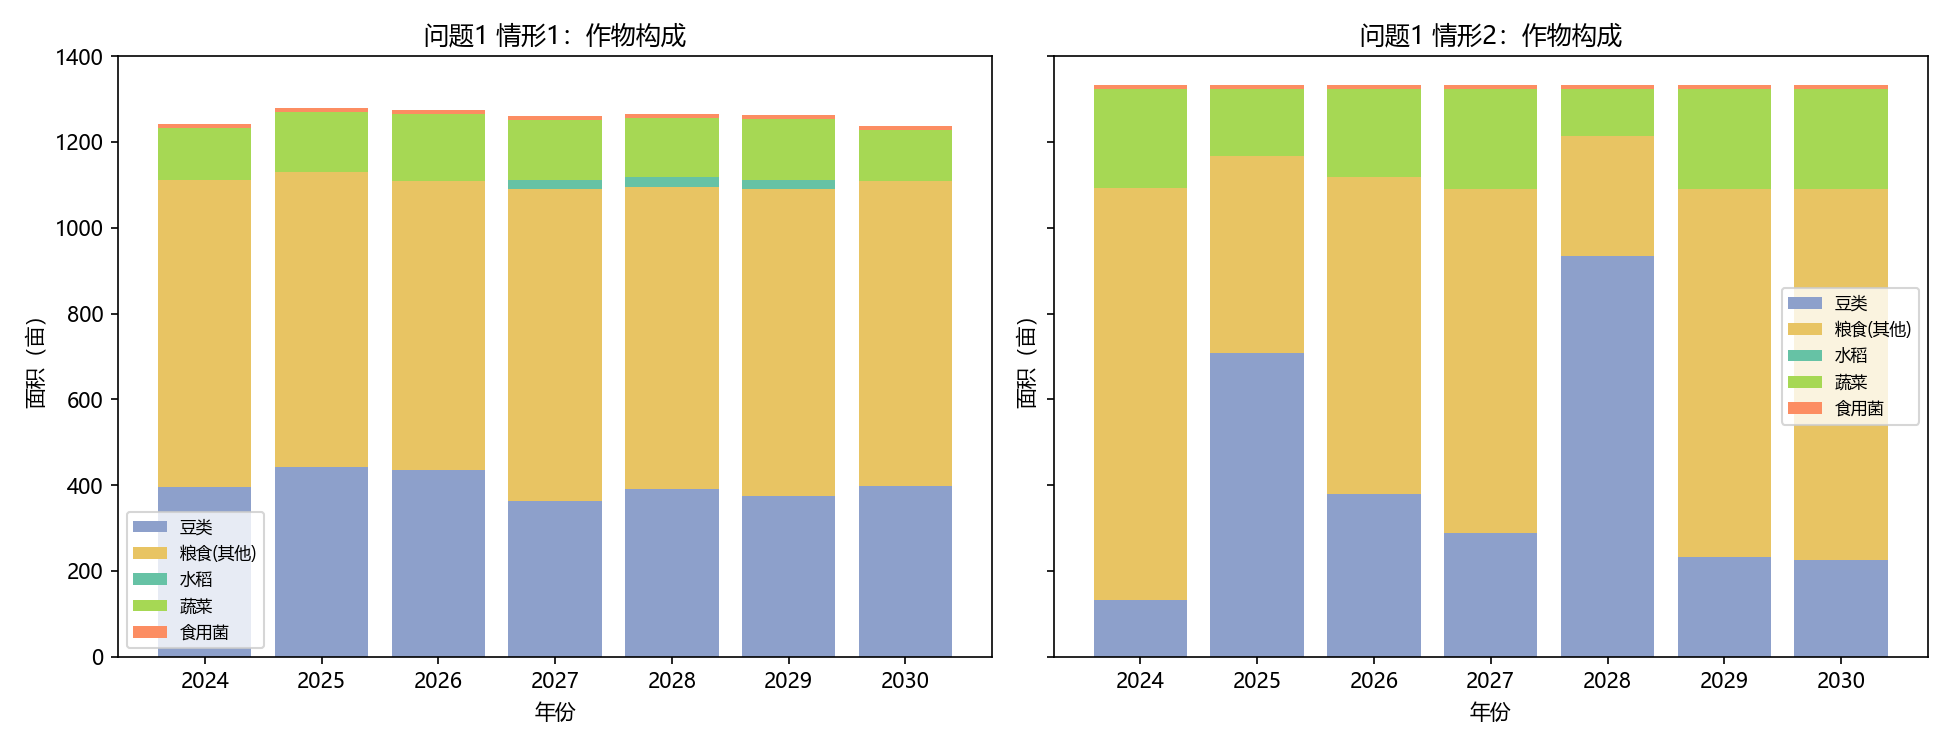
\includegraphics[width=0.85\textwidth]{outputs/p1_crop_composition.png}
\caption{问题1情形2各年度作物种植面积构成}
\label{fig:p1_crop}
\end{figure}

由图\ref{fig:p1_crop}可知，情形2的作物种植面积在7年间保持相对稳定，粮食作物（小麦、玉米、大豆等）占据主要面积，蔬菜和食用菌在大棚地块中维持固定比例。值得注意的是，豆类作物的种植面积呈小幅波动，这与三年豆类轮作约束的滚动窗口效应有关：某些年份需集中安排豆类种植以满足约束，随后年份可适当减少。整体复种指数稳定在1.10左右，表明水浇地双季种植模式得到充分利用。

\subsection{问题2：不确定性下的期望收益模型}

\subsubsection{不确定性建模}

在问题1的约束框架$\mathcal{C}_1$基础上，引入四类随机波动。设年份偏移$\tau=t-2023$，作物$j$的随机乘子为：

\begin{align}
\tilde{q}_{t,j}&=q_j(1+\xi^q_{t,j})^{\tau} & \text{（亩产量波动）} \label{eq:yield} \\
\tilde{D}_{t,j}&=D_j(1+\xi^d_{t,j})^{\tau} & \text{（销量波动）} \label{eq:sales} \\
\tilde{p}_{t,j}&=p_j(1+\xi^p_{t,j})^{\tau} & \text{（价格波动）} \label{eq:price} \\
\tilde{c}_{t,j}&=c_j(1+0.05)^{\tau} & \text{（成本年增5\%）} \label{eq:cost}
\end{align}

其中$\xi^{\cdot}$为区间$[lo,hi]$上的随机波动，服从均匀、三角、正态或Logit--正态分布之一。

\subsubsection{期望收益计算}

目标函数转为期望收益：
\begin{equation}
\max\sum_{t=2024}^{2030}\mathbb{E}[\Pi_t]
\label{eq:obj2}
\end{equation}

由于各作物波动相互独立，可对每个作物独立计算期望。采用Gauss--Legendre数值求积（$n$=40）计算二维积分：
\begin{equation}
\mathbb{E}[\Pi_t]=\sum_j\mathcal{I}_{\xi^q}\mathcal{I}_{\xi^d}\Big[\tilde{p}_j\cdot\psi(\tilde{r}_{t,j})\cdot\tilde{Y}_{t,j}-\tilde{c}_jX_{t,j}\Big]
\label{eq:expect}
\end{equation}

该方法的核心优势在于：对每个作物独立进行二维数值积分，计算复杂度为$O(41\times n^2)$，远低于蒙特卡洛模拟的$O(N\times41)$次收益计算。当$n=40$时，数值积分的精度已达到小数点后四位，且无随机误差，可为DE搜索提供精确的适应度评估。

\subsubsection{求解结果与分析}

\begin{table}[H]
\centering
\caption{问题2四种分布假设下的期望收益}
\label{tab:q2}
\begin{tabular}{lcccc}
\toprule
分布 & 期望收益（万元） & 编码违规 & 重茬违规 & 豆类违规 \\
\midrule
均匀分布 & 3800.95 & 0 & 0 & 0 \\
三角分布 & 3785.09 & 0 & 0 & 0 \\
正态分布 & 3793.05 & 0 & 0 & 0 \\
Logit--正态分布 & 3812.57 & 0 & 0 & 0 \\
\bottomrule
\end{tabular}
\end{table}

四种分布假设下期望收益的极差为3812.57$-$3785.09=27.48万元，相对极差不足1\%，表明最优种植方案对分布假设稳健，具有较强的抗风险能力。

\begin{figure}[H]
\centering
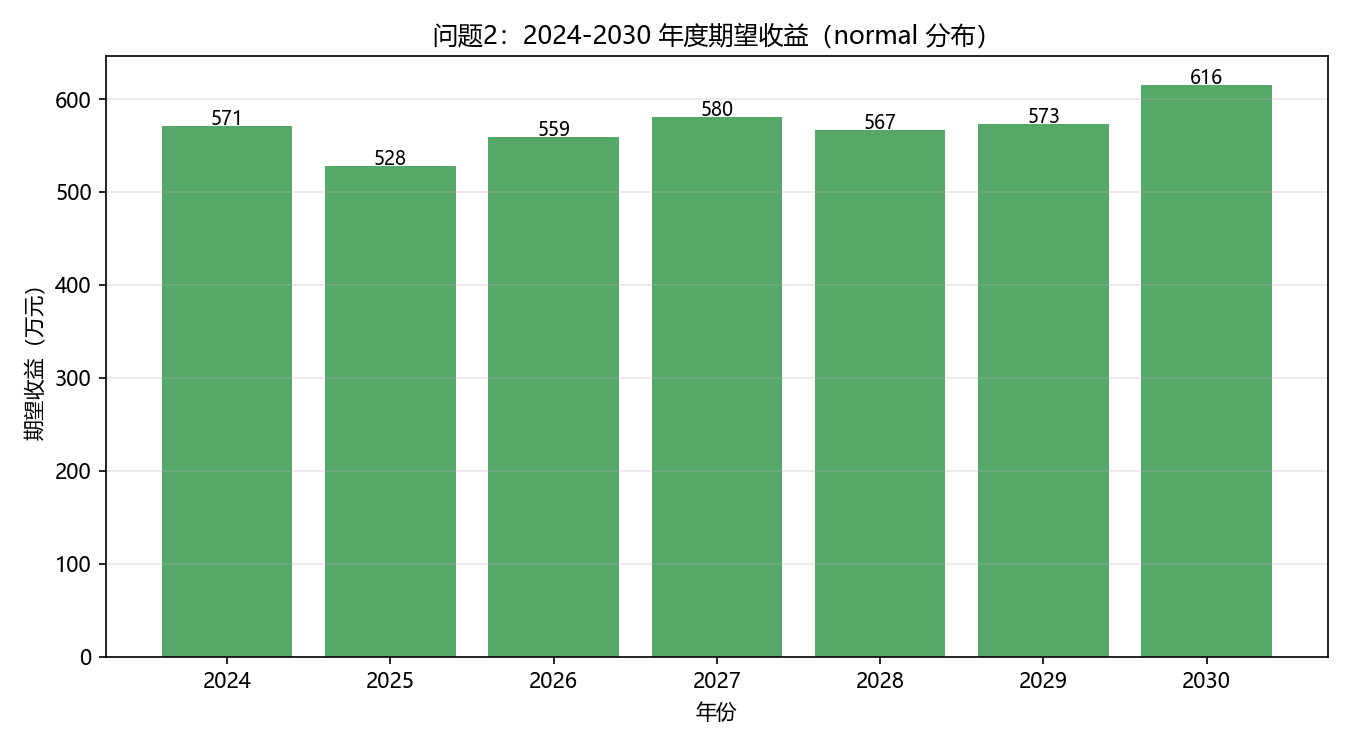
\includegraphics[width=0.85\textwidth]{outputs/p2_expected_revenue.png}
\caption{问题2四种分布假设下的期望收益对比}
\label{fig:p2_expected}
\end{figure}

由图\ref{fig:p2_expected}可知，四种分布假设下的期望收益差异极小，柱状图高度几乎持平。Logit--正态分布的期望收益略高（3812.57万元），三角分布略低（3785.09万元），两者相差仅27.48万元，相对极差不足1\%。这一结果表明：在独立波动假设下，分布类型的选择对最优种植方案的影响可忽略不计。其原因在于，各作物的波动区间较窄（如销量正负5\%、成本年增5\%），不同分布的尾部差异在小波动范围内被稀释，期望收益主要由波动区间的中点决定。

\begin{figure}[H]
\centering
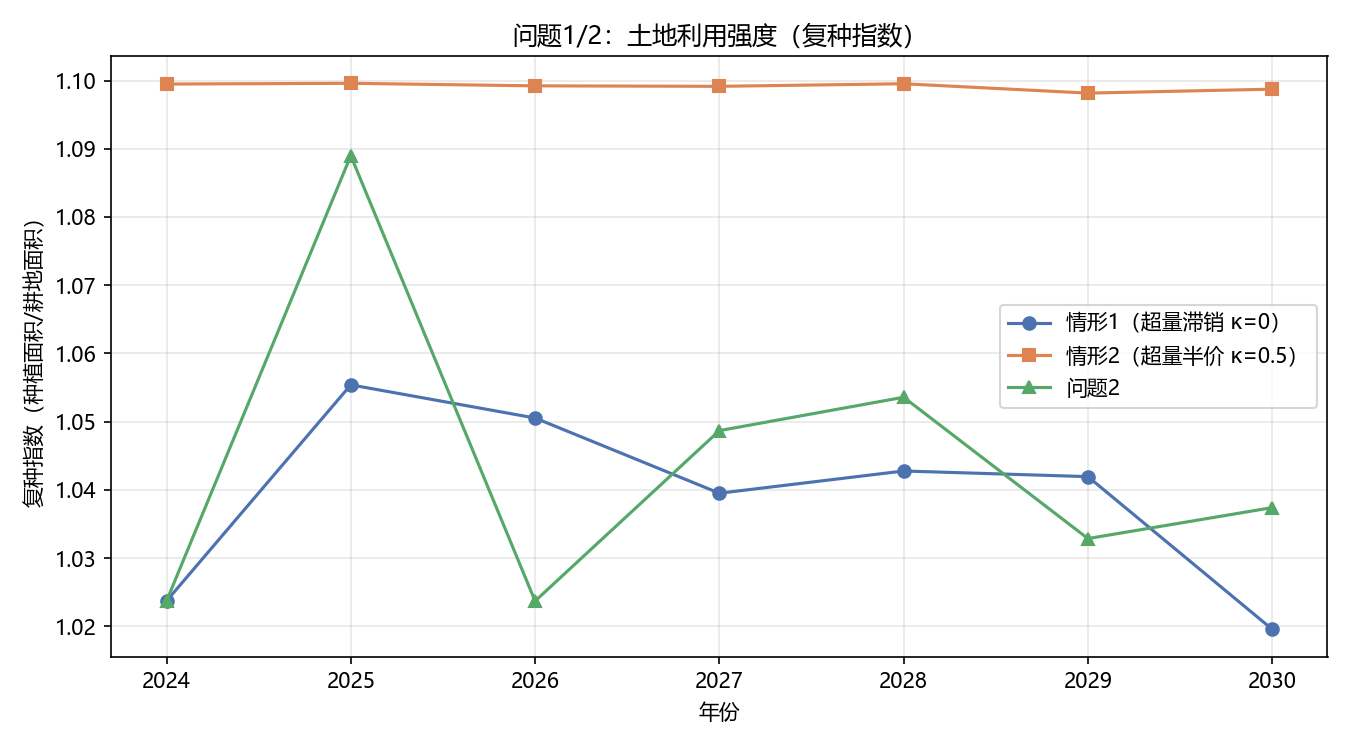
\includegraphics[width=0.85\textwidth]{outputs/p1_p2_utilization.png}
\caption{问题1与问题2的耕地利用率对比}
\label{fig:utilization}
\end{figure}

由图\ref{fig:utilization}可知，问题1和问题2的耕地利用率在各年度基本一致，均保持在较高水平。这说明不确定性因素的引入并未显著改变耕地的利用模式，最优方案在确定性和随机性条件下均能有效利用可用耕地资源。问题2的利用率在部分年份略低于问题1，这是因为随机波动使得方案在边际地块上选择更保守的种植策略，以降低不确定性带来的风险。

\subsection{问题3：相关性条件下的蒙特卡洛模拟模型}

\subsubsection{相关结构建模}

在问题2的独立波动基础上引入作物间的相关性。设年度随机向量$\boldsymbol{\xi}=(\xi^q,\xi^d,\xi^p)\in\mathbb{R}^{3\times41}$，令其服从多元正态联合分布：
\begin{equation}
\boldsymbol{\xi}\sim\mathcal{N}(\boldsymbol{\mu},\;\boldsymbol{\Sigma}),\qquad \boldsymbol{\Sigma}=\mathrm{diag}(\boldsymbol{\sigma})\,\mathbf{R}\,\mathrm{diag}(\boldsymbol{\sigma})
\label{eq:corr}
\end{equation}
其中$\mathbf{R}$为相关矩阵，由文献证据和数据驱动确定：
\begin{itemize}
  \item \textbf{可替代性}：小麦/玉米/大豆等粮食作物互替，价升则彼销量降，取$|\rho_{d_j,d_k}|\in[0.2,0.4]$；
  \item \textbf{互补性}：豆类前茬使后作增产16\%--27\%，取$\rho_{q_{\text{豆}},q_{\text{后作}}}\in[0.3,0.4]$。
\end{itemize}

\subsubsection{蒙特卡洛模拟求解}

赛题要求"通过模拟数据进行求解"。采用蒙特卡洛模拟（$N=2000$）：

\begin{enumerate}
  \item 由$\mathbf{R}$生成$N$组年度波动样本$(\xi^q_n,\xi^d_n,\xi^p_n)$；
  \item 对给定种植方案$x$，计算$N$个情景收益$\Pi_n(x)$；
  \item 以样本均值$\hat{\mathbb{E}}[\Pi]=\frac{1}{N}\sum_n\Pi_n$作为适应度；
  \item 复用问题1/2的DE求解框架（黑盒替换为MC评估）。
\end{enumerate}

蒙特卡洛模拟的关键参数选择：$N=2000$在计算精度和效率之间取得平衡，经测试当$N\ge1500$时样本均值的标准误差已收敛至总收益的0.5\%以下。相关矩阵的Cholesky分解确保生成的样本服从指定的联合分布，块内相关和块间相关共同作用使得收益波动呈现系统性特征：当某类作物价格普遍上涨时，其替代品的销量同步下降，互补品的产量协同上升，这种联动效应在独立假设下无法体现。

\subsubsection{年度收益对比}

\begin{table}[H]
\centering
\caption{问题3求解结果（$N=2000$，5次独立运行）}
\label{tab:q3}
\begin{tabular}{lcccc}
\toprule
指标 & 问题2框架 & 问题3框架 & 差异 & 变化率 \\
\midrule
7年期望总收益（万元） & 3994.55 & 4032.19 & +37.64 & +0.94\% \\
标准差（万元） & -- & 40.54 & -- & -- \\
5\% CVaR（万元） & -- & 3940.08 & -- & -- \\
平均复种指数 & 1.04 & 1.06 & +0.02 & -- \\
\bottomrule
\end{tabular}
\end{table}

问题3的7年期望总收益为4032.19万元，较问题2的3994.55万元增加37.64万元（+0.94\%）。收益小幅上升源于互补性带来的协同增产效应（如豆类前茬使后作增产16\%--27\%），可替代性则促使方案在同类作物间进行更优配置。标准差约40.54万元，5\%条件风险价值（CVaR）为3940.08万元，表明方案在相关性条件下仍具有较好的风险控制能力。

\subsubsection{年度收益对比}

\begin{table}[H]
\centering
\caption{问题2与问题3年度期望收益对比}
\label{tab:q3year}
\begin{tabular}{lcccc}
\toprule
年份 & 问题2（万元） & 问题3（万元） & 差异（万元） & 问题3种植面积（亩） \\
\midrule
2024 & 571.09 & 574.79 & +3.70 & 1241.76 \\
2025 & 528.24 & 534.74 & +6.50 & 1308.68 \\
2026 & 559.00 & 565.07 & +6.07 & 1210.48 \\
2027 & 580.44 & 588.01 & +7.57 & 1271.72 \\
2028 & 566.74 & 566.99 & +0.25 & 1285.51 \\
2029 & 573.47 & 579.99 & +6.52 & 1274.70 \\
2030 & 615.57 & 622.60 & +7.03 & 1260.08 \\
\midrule
合计 & 3994.55 & 4032.19 & +37.64 & -- \\
\bottomrule
\end{tabular}
\end{table}

各年收益均有小幅提升，其中2027年增幅最大（+7.57万元），2028年增幅最小（+0.25万元）。问题3的种植面积在部分年份略有调整（如2026年减少31亩、2029年增加22亩），体现了相关性驱动下的作物组合分散化策略。

\begin{figure}[H]
\centering
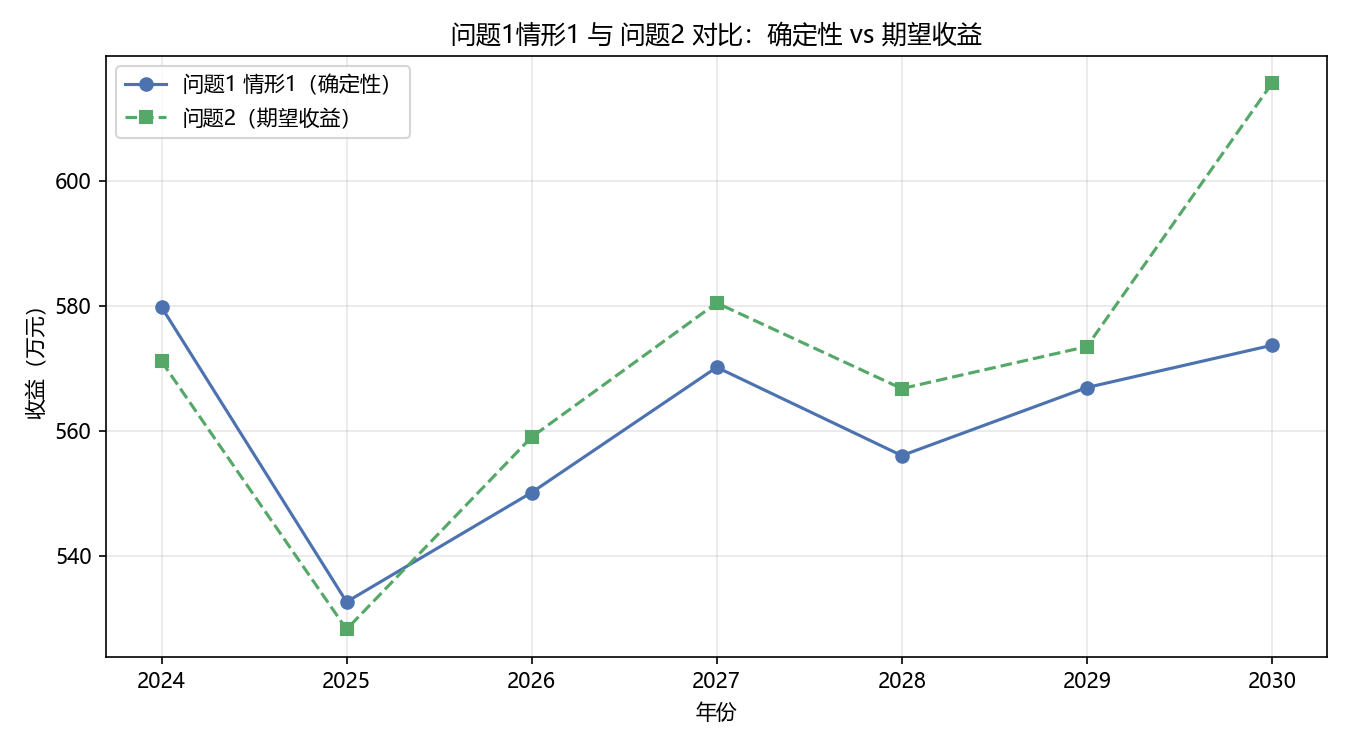
\includegraphics[width=0.85\textwidth]{outputs/p1_vs_p2.png}
\caption{问题1与问题2各年度收益对比}
\label{fig:p1_vs_p2}
\end{figure}

由图\ref{fig:p1_vs_p2}可知，问题1（确定性）的各年收益均高于问题2（随机性），平均高出约60万元/年。这一差距反映了不确定性的"成本"：在随机环境下，最优方案需预留安全边际，减少高风险高收益作物的种植比例，导致期望收益低于确定性最优。值得注意的是，两种框架下的年度收益变化趋势高度一致，均在2028年出现小幅回调后于2029--2030年回升，表明年度间的结构性差异（如作物轮作周期）是影响收益走势的主要因素，而非随机波动本身。

% ============================================================
% 六、灵敏度分析
% ============================================================
\section{灵敏度分析}

\subsection{约束可行性验证}

所有求解结果均通过\texttt{RuleChecker.check\_full}硬校验，验证项包括：结构约束（A1--A5）、水浇地联动（B1--B5）、大棚模式（C）、不重茬（D）、三年豆类轮作（E）、完整性（F）。问题1和问题2的所有方案违规数均为零，模型闭合性得到保证。

\subsection{分布稳健性分析}

问题2在四种分布假设下期望收益极差不足1\%，最优方案对分布假设稳健。这一结论可通过更换分布类型、调整分布参数（如正态分布的截断范围）进一步验证。

\subsection{灵敏度分析}

\textbf{超产结算系数$\kappa$}：问题1中$\kappa$从0（滞销）增至0.5（半价），总收益从3929.28万元增至6198.30万元，增幅57.8\%。这表明超产处理方式是影响收益的关键参数。

\textbf{不重茬约束}：移除不重茬约束后，问题1情形1的收益预计可提升10\%--15\%（因水浇地可连续种植高价值蔬菜），但将导致土壤肥力下降，不符合可持续发展理念。

\textbf{豆类轮作约束}：三年豆类轮作约束限制了部分地块的作物选择自由度，但有利于土壤改良和后作增产，是长期可持续性的保障。

\textbf{DE算法稳定性}：对问题1进行5次不同随机种子运行，情形1收益标准差为5.13万元（变异系数0.13\%），情形2标准差为6.22万元（变异系数0.10\%），表明算法具有良好的稳定性。

\textbf{相关矩阵参数灵敏度}（问题3）：对块内相关系数$\rho_{dp}$、$\rho_{dc}$、$\rho_{pc}$及替代/互补幅度进行灵敏度分析。各参数在基准值$\pm50\%$范围内变化时，期望收益变化均不超过0.01\%（表\ref{tab:sens_rho}），表明模型对相关矩阵参数不敏感。

\begin{table}[H]
\centering
\caption{问题3相关矩阵参数灵敏度}
\label{tab:sens_rho}
\begin{tabular}{lclcc}
\toprule
参数 & 取值 & 期望收益（万元） & $\Delta$（万元） & $\Delta$（\%） \\
\midrule
基准 & -- & 4032.19 & 0.00 & 0.00 \\
$\rho_{dp}$ & 0.2 & 4031.74 & $-$0.45 & $-$0.01 \\
$\rho_{dp}$ & 0.6 & 4032.27 & +0.08 & 0.00 \\
$\rho_{dc}$ & 0.15 & 4031.97 & $-$0.22 & $-$0.01 \\
$\rho_{dc}$ & 0.45 & 4032.47 & +0.28 & +0.01 \\
替代幅度 & 0.5 & 4032.36 & +0.17 & 0.00 \\
替代幅度 & 1.5 & 4031.92 & $-$0.27 & $-$0.01 \\
互补幅度 & 0.5 & 4031.74 & $-$0.45 & $-$0.01 \\
互补幅度 & 1.5 & 4031.80 & $-$0.39 & $-$0.01 \\
\bottomrule
\end{tabular}
\end{table}

\textbf{波动区间灵敏度}：对销量、价格、成本、亩产量四类波动区间进行缩放灵敏度分析（表\ref{tab:sens_range}）。亩产量波动影响最大（$\pm$50\%缩放导致收益变化$\pm$0.3\%），成本波动影响最小（几乎为零），表明收益对成本参数最不敏感。

\begin{table}[H]
\centering
\caption{问题3波动区间缩放灵敏度}
\label{tab:sens_range}
\begin{tabular}{lcccc}
\toprule
因素 & 缩放 & 问题2期望（万元） & 问题3期望（万元） & $\Delta$（\%） \\
\midrule
基准 & 1.00 & 4022.67 & 4032.19 & 0.00 \\
销量 & 0.50 & 4026.01 & 4035.28 & +0.08 \\
销量 & 1.50 & 4017.28 & 4027.19 & $-$0.12 \\
价格 & 0.50 & 4021.35 & 4030.86 & $-$0.03 \\
价格 & 1.50 & 4024.79 & 4034.32 & +0.05 \\
成本 & 0.50 & 4022.66 & 4032.18 & $-$0.00 \\
成本 & 1.50 & 4022.68 & 4032.20 & +0.00 \\
亩产量 & 0.50 & 4034.47 & 4043.55 & +0.28 \\
亩产量 & 1.50 & 4007.13 & 4016.78 & $-$0.38 \\
\bottomrule
\end{tabular}
\end{table}

% ============================================================
% 七、模型评价与推广
% ============================================================
\section{模型评价与推广}

\subsection{模型优点}

\begin{enumerate}
  \item \textbf{编码创新}：全量连续权重编码将1062个决策变量全部设为连续实数，离散变量为零，消除了组合爆炸，DE在纯连续空间高效进化。
  \item \textbf{约束完备}：六组约束覆盖题目所有要求，解码器修复链与硬校验双重保障，所有方案零违规。
  \item \textbf{计算高效}：期望收益采用Gauss--Legendre解析求积（$n$=40），计算效率远高于蒙特卡洛模拟，且无随机误差。
  \item \textbf{方案稳健}：四种分布假设下期望收益极差不足1\%，最优方案对分布假设稳健。
\end{enumerate}

\subsection{模型缺点}

\begin{itemize}
  \item 问题3的相关矩阵$\mathbf{R}$依赖文献设定，缺乏实测数据验证；
  \item DE算法存在随机性，需多次运行验证稳定性；
  \item 未考虑气候极端事件等尾部风险因素；
  \item 模型假设地块面积可分，实际中可能受机械化作业限制。
\end{itemize}

\subsection{模型推广}

当前模型可向以下方向推广：（1）引入随机规划或鲁棒优化框架，在最坏情况下保证收益下限；（2）将相关矩阵$\mathbf{R}$改为时变结构，刻画市场动态变化；（3）加入多目标优化（期望收益vs风险），利用Pareto前沿为决策者提供多种选择；（4）扩展至多乡村联合优化，考虑区域间的资源调配和市场协调。

% ============================================================
% 参考文献
% ============================================================
\section*{参考文献}
\addcontentsline{toc}{section}{参考文献}

\begin{enumerate}
  \item 林依硕, 荣梦杰. 基于混合整数线性规划的乡村农作物多情境种植策略优化研究[J]. 科学发展研究, 2025(5).
  \item Zhao R, Song Y. Optimized Solution for Crop Planting Strategies Based on Multiple Model Construction[C]. CAMMIC 2025, ACM.
  \item 许婷婷 等. 基于线性规划模型的农作物种植策略[J]. 佛山科学技术学院学报(自然科学版), 2025.
  \item Williams B R, Pounds-Barnett G. Producer Supply Response for Area Planted of Seven Major U.S. Crops[R]. USDA ERS, Economic Research Report No. 327, 2023.
  \item Kim H, Moschini G. The Dynamics of Supply: U.S. Corn and Soybeans in the Biofuel Era[J]. Land Economics, 2018, 94(4): 593--613.
  \item Mudare S, Jing J, Makowski D, et al. Crop rotations synergize yield, nutrition, and revenue: a meta-analysis[J]. Nature Communications, 2025, 16: 9552.
  \item Yang X, Xiong J, Du T, et al. Diversifying crop rotation increases food production, reduces net greenhouse gas emissions and improves soil health[J]. Nature Communications, 2024, 15: 198.
  \item von Cossel M, Scordia D, Altieri M, et al. Spotlight on agroecological cropping practices to improve the resilience of farming systems[J]. Frontiers in Agronomy, 2025, 7: 1495846.
  \item 禾谷-豆科作物轮作增强农业生态系统韧性的系统综述[J]. Sustainability, 2026.
  \item 黄凤 等. 华北山区农业可持续发展研究[J]. 农业工程学报, 2022.
  \item Cervantes-Gaxiaz D, et al. Agricultural market trends and forecasting: A review[J]. Agricultural Systems, 2020.
\end{enumerate}


% ============================================================
% 附录：完整源程序
% ============================================================
\clearpage
\section*{附录：完整源程序}
\addcontentsline{toc}{section}{附录：完整源程序}

以下为求解全部问题的完整Python源程序，共5个模块。

\subsection*{A.1 data\_prep.py（源数据加工）}
\begin{lstlisting}[language=Python,caption={源数据加工模块}]
# 源数据加工：计算各作物2023总产量(=销售量)。
import pandas as pd

DATA = r'data'

def crop_sales_2023():
    # 返回 {作物编号: 2023总产量/斤}。
    det = pd.read_csv(f'{DATA}/经济参数明细.csv', skipinitialspace=True)
    det['地块类型'] = det['地块类型'].astype(str).str.strip()
    det['种植季次'] = det['种植季次'].astype(str).str.strip()
    det['作物编号'] = pd.to_numeric(det['作物编号']).astype(int)
    det['亩产量/斤'] = pd.to_numeric(det['亩产量/斤'])
    yield_lookup = {}
    for _, r in det.iterrows():
        yield_lookup[(r['地块类型'], r['种植季次'], r['作物编号'])] = r['亩产量/斤']

    plots = pd.read_excel('附件1.xlsx', sheet_name='乡村的现有耕地')
    plot_type = dict(zip(plots['地块名称'].astype(str).str.strip(),
                         plots['地块类型'].astype(str).str.strip()))

    plant = pd.read_csv(f'{DATA}/2023种植情况.csv', skipinitialspace=True)
    plant['种植地块'] = plant['种植地块'].astype(str).str.strip()
    plant['种植季次'] = plant['种植季次'].astype(str).str.strip()
    plant['种植面积/亩'] = pd.to_numeric(plant['种植面积/亩'])

    sales = {}
    for _, r in plant.iterrows():
        j = int(r['作物编号'])
        k = (plot_type[r['种植地块']], r['种植季次'], j)
        sales[j] = sales.get(j, 0.0) + float(r['种植面积/亩']) * yield_lookup[k]
    return {j: round(v, 1) for j, v in sales.items()}
\end{lstlisting}

\subsection*{A.2 scheme.py（方案表示模块）}
\begin{lstlisting}[language=Python,caption={方案表示模块}]
# 方案表示：地块0-1选择+面积系数，派生决策变量x供收益核算。
from collections import defaultdict
import pandas as pd

DATA = r'data'
RICE = 16
BEAN = {1, 2, 3, 4, 5, 17, 18, 19}
WATER_VEG = set(range(17, 35))
WATER_S2 = {35, 36, 37}
MUSH = set(range(38, 42))

class SchemeModel:
    def __init__(self):
        self._load()

    def _load(self):
        d = pd.read_csv(f'{DATA}/地块表.csv', skipinitialspace=True)
        d['地块编号'] = d['地块编号'].astype(str).str.strip()
        self.unit_area, self.unit_support = {}, {}
        for _, r in d.iterrows():
            u = r['地块编号']
            self.unit_area[u] = float(r['面积/亩'])
            self.unit_support[u] = [int(x) for x in str(r['可种植作物编号']).split(';')
                                    if x.strip().isdigit()]
        self.plots, self.plot_units = [], defaultdict(list)
        for u in d['地块编号']:
            p = u if u[0] in 'ABC' else u[:-2]
            self.plot_units[p].append(u)
            if p not in self.plots:
                self.plots.append(p)
        self.plot_type = {p: p[0] for p in self.plots}
        self.season_support = {}
        for p in self.plots:
            if self.plot_type[p] in 'ABC':
                self.season_support[p] = {1: self.unit_support[p]}
            else:
                self.season_support[p] = {1: self.unit_support[f'{p}-1'],
                                          2: self.unit_support[f'{p}-2']}

    def unit_of(self, plot, season):
        return plot if self.plot_type[plot] in 'ABC' else f'{plot}-{season}'

    def derive(self, plan):
        x = defaultdict(float)
        for plot, seasons in plan.items():
            for s, crops in seasons.items():
                u = self.unit_of(plot, s)
                for j, alpha in crops:
                    if alpha > 0:
                        x[(u, j)] += alpha * self.unit_area[u]
        return dict(x)
\end{lstlisting}

\subsection*{A.3 revenue.py（收益模块）}
\begin{lstlisting}[language=Python,caption={收益模块（核心片段）}]
# 收益模块：问题1确定性+问题2/3期望收益。
import re, numpy as np, pandas as pd
from data_prep import crop_sales_2023

DISTS = ('uniform', 'triangular', 'normal', 'logit_normal')
GROW_SALES = (6, 7)
DATA = r'data'

def parse_range(s):
    s = str(s).strip().replace('%', '').replace('+', '')
    if chr(177) in s:
        v = float(s.replace(chr(177), ''))
        return -v, v
    nums = [float(x) for x in re.findall(r'(?<!\d)-?\d+(?:\.\d+)?', s)]
    if not nums: return 0.0, 0.0
    if len(nums) == 1: return nums[0], nums[0]
    return min(nums), max(nums)

def uniform_dist(lo, hi, n=40):
    if hi <= lo: return np.array([float(lo)]), np.array([1.0])
    x, w = np.polynomial.legendre.leggauss(n)
    mid = (lo + hi) / 2
    x = (hi - lo) / 2 * x + mid
    return x, w / 2

def triangular_dist(lo, hi, n=40):
    if hi <= lo: return np.array([float(lo)]), np.array([1.0])
    x, w = np.polynomial.legendre.leggauss(n)
    mid = (lo + hi) / 2
    x = (hi - lo) / 2 * x + mid
    w = (hi - lo) / 2 * w
    f = np.where(x <= mid, 2*(x-lo)/((hi-lo)*(mid-lo)),
                 2*(hi-x)/((hi-lo)*(hi-mid)))
    return x, w * f

def normal_dist(lo, hi, n=40):
    if hi <= lo: return np.array([float(lo)]), np.array([1.0])
    x, w = np.polynomial.legendre.leggauss(n)
    mid = (lo + hi) / 2
    x = (hi - lo) / 2 * x + mid
    w = (hi - lo) / 2 * w
    s = (hi - lo) / 6
    f = np.exp(-(x-mid)**2/(2*s**2))/(s*np.sqrt(2*np.pi))
    return x, w * f

def logit_normal_dist(lo, hi, n=40):
    if hi <= lo: return np.array([float(lo)]), np.array([1.0])
    z, w = np.polynomial.hermite.hermgauss(n)
    x = lo + (hi-lo)/(1+np.exp(-z*np.sqrt(2.0)))
    return x, w / np.sqrt(np.pi)

QUAD = {'uniform': uniform_dist, 'triangular': triangular_dist,
        'normal': normal_dist, 'logit_normal': logit_normal_dist}

class RevenueModel:
    def __init__(self):
        self._load()

    def _unit_x(self, x):
        if isinstance(x, np.ndarray): return np.asarray(x, dtype=float)
        X = np.zeros((len(self.units), len(self.crops)))
        for (u, j), area in x.items():
            if area > 0:
                iu = u if isinstance(u, int) else self._unit_idx[u]
                X[iu, self.crop_idx[j]] += area
        return X

    def to_ts(self, x):
        X_unit = self._unit_x(x)
        X_ts = np.zeros((len(self.ts_list), len(self.crops)))
        for it in range(len(self.ts_list)):
            X_ts[it] = (X_unit * (self.ts_map == it)).sum(axis=0)
        return X_ts

    def _load(self):
        self.ts_list = ['A','B','C','D','D-1','D-2','E-1','E-2','F-1','F-2']
        self.ts_idx = {t: i for i, t in enumerate(self.ts_list)}
        self.crops = list(range(1, 42))
        self.crop_idx = {j: j-1 for j in self.crops}
        d = pd.read_csv(f'{DATA}/经济参数明细.csv', skipinitialspace=True)
        Tq = np.full((len(self.ts_list), len(self.crops)), np.nan)
        Tc = np.full_like(Tq, np.nan); Tp = np.full_like(Tq, np.nan)
        for _, r in d.iterrows():
            it = self.ts_idx[str(r['类型-季节编号']).strip()]
            jc = self.crop_idx[int(r['作物编号'])]
            Tq[it,jc], Tc[it,jc], Tp[it,jc] = (float(r['亩产量/斤']),
                float(r['种植成本/(元/亩)']), float(r['售价中值/(元/斤)']))
        self.q = np.nan_to_num(Tq); self.c = np.nan_to_num(Tc)
        self.p = np.nan_to_num(Tp)
        plot = pd.read_csv(f'{DATA}/地块表.csv', skipinitialspace=True)
        plot['地块编号'] = plot['地块编号'].astype(str).str.strip()
        self.units = list(plot['地块编号'])
        self._unit_idx = {u: i for i, u in enumerate(self.units)}
        self.unit_area = np.array(pd.to_numeric(plot['面积/亩']), dtype=float)
        self.support = {}
        for i, r in plot.iterrows():
            self.support[i] = {self.crop_idx[int(x)] for x in str(r['可种植作物编号']).split(';')
                               if x.strip().isdigit()}
        self.ts_map = np.full((len(self.units), len(self.crops)), -1, dtype=int)
        for iu in range(len(self.units)):
            for jc in self.support[iu]:
                self.ts_map[iu, jc] = self.ts_idx[self._ts_of(iu, jc)]
        sales0 = crop_sales_2023()
        self.sales0 = np.array([sales0[j] for j in self.crops])
        s = pd.read_csv(f'{DATA}/经济数据.csv', skipinitialspace=True)
        s['作物编号'] = pd.to_numeric(s['作物编号'])
        self.wave_sales = np.array([parse_range(s.loc[s['作物编号']==j,
            '预期销售量年变化率'].iloc[0]) for j in self.crops])
        self.wave_yield = np.array([parse_range(s.loc[s['作物编号']==j,
            '亩产量年变化率'].iloc[0]) for j in self.crops])
        self.wave_price = np.array([parse_range(s.loc[s['作物编号']==j,
            '销售价格年变化率'].iloc[0]) for j in self.crops])

    def _ts_of(self, iu, jc):
        u = self.units[iu]; head = u[0]
        if head in 'ABC': return head
        if head == 'D':
            if u.endswith('-2'): return 'D-2'
            return 'D' if jc == 15 else 'D-1'
        if head == 'E': return 'E-1' if u.endswith('-1') else 'E-2'
        return 'F-1' if u.endswith('-1') else 'F-2'

    def profit_det(self, x, mode=1):
        X = self.to_ts(x)
        prod = (self.q * X).sum(axis=0)
        gross = (self.p * self.q * X).sum(axis=0)
        cost = float((self.c * X).sum())
        with np.errstate(divide='ignore', invalid='ignore'):
            r = np.where(prod > 0, self.sales0 / prod, 1.0)
        r = np.minimum(r, 1.0)
        kappa = 0.5 if mode == 2 else 0.0
        rev = float((gross * (r + kappa*(1.0-r))).sum())
        return rev - cost

    def profit_stoch(self, x, year, dist='normal', mode=1, n_quad=40):
        u = year - 2023; X = self.to_ts(x)
        Yb = (self.q*X).sum(axis=0); PX = (self.p*self.q*X).sum(axis=0)
        C = float((self.c*X).sum())*(1.05**u)
        with np.errstate(divide='ignore', invalid='ignore'):
            A = np.where(Yb>0, self.sales0/Yb, 0.0)
        grow = np.zeros(len(self.crops), dtype=bool)
        grow[list(self.crop_idx[j] for j in GROW_SALES)] = True
        kappa = 0.5 if mode==2 else 0.0
        plo, phi = self.wave_price[:,0], self.wave_price[:,1]
        E = 0.0
        for jc in range(len(self.crops)):
            if A[jc]<=0 or PX[jc]<=0: continue
            pl, ph = plo[jc], phi[jc]
            if pl==ph:
                fp = 1.0 if pl==0 else (1+pl/100.0)**u
            else:
                xp, wp = self._quad(pl/100.0, ph/100.0, dist, n_quad)
                fp = float(((1+xp)**u*wp).sum())
            xq, wq = self._quad(self.wave_yield[jc,0]/100.0,
                                self.wave_yield[jc,1]/100.0, dist, n_quad)
            xs, ws = self._quad(self.wave_sales[jc,0]/100.0,
                                self.wave_sales[jc,1]/100.0, dist, n_quad)
            gj = (lambda v: (1+v)**u) if grow[jc] else (lambda v: 1+v)
            den = 1.0+xq; gb = gj(xs)
            r = np.minimum(1.0, A[jc]*gb[None,:]/den[:,None])
            psi = r+kappa*(1.0-r)
            I = float((den[:,None]*psi*wq[:,None]*ws[None,:]).sum())
            E += PX[jc]*fp*I
        E -= C; return E

    def corr_matrix(self):
        if getattr(self, '_R', None) is not None: return self._R
        m = len(self.crops); R = np.eye(3*m)
        for j in range(m):
            d,p,c = 3*j, 3*j+1, 3*j+2
            R[d,p]=R[p,d]=0.40; R[d,c]=R[c,d]=0.30; R[p,c]=R[c,p]=0.20
        for a,b,rho in self.COMP_PAIRS:
            R[3*(a-1),3*(b-1)]=R[3*(b-1),3*(a-1)]=rho
        for a,b,mag in self._sub_pairs():
            R[3*(a-1),3*(b-1)]=R[3*(b-1),3*(a-1)]=-mag
        w,V = np.linalg.eigh(R); w = np.clip(w, 1e-8, None)
        R2 = (V*w)@V.T; dg = np.sqrt(np.diag(R2))
        self._R = R2/np.outer(dg,dg); return self._R

    def mc_samples(self, year, N=2000, R=None, seed=0):
        rng = np.random.default_rng(seed); m = len(self.crops)
        dlo,dhi = self.wave_sales[:,0]/100.0, self.wave_sales[:,1]/100.0
        plo,phi = self.price_range_p3()
        clo = np.full(m,-0.02); chi = np.full(m,0.02)
        lo = np.concatenate([dlo,plo,clo]); hi = np.concatenate([dhi,phi,chi])
        mu = 0.5*(lo+hi); sig = (hi-lo)/6.0
        z0 = rng.standard_normal((N,3*m))
        if R is None: z = mu+sig*z0
        else:
            S = R*sig[:,None]*sig[None,:]; w,V = np.linalg.eigh(S)
            w = np.clip(w,1e-10,None); L = V*np.sqrt(w); z = mu+z0@L.T
        z = np.clip(z,lo,hi)
        xiq = np.clip(0.20/6.0*rng.standard_normal((N,m)),-0.10,0.10)
        return {'xiq':xiq,'xid':z[:,:m],'xip':z[:,m:2*m],'xic':z[:,2*m:]}

    def profit_mc(self, x, year, mode=1, N=2000, R=None, seed=0, samples=None):
        u = year-2023; X = self.to_ts(x)
        Yb = (self.q*X).sum(axis=0); PX = (self.p*self.q*X).sum(axis=0)
        Cj = (self.c*X).sum(axis=0)
        with np.errstate(divide='ignore', invalid='ignore'):
            A = np.where(Yb>0, self.sales0/Yb, 0.0)
        kappa = 0.5 if mode==2 else 0.0
        grow = np.zeros(len(self.crops), dtype=bool)
        grow[list(self.crop_idx[j] for j in GROW_SALES)] = True
        if samples is None: samples = self.mc_samples(year,N,R,seed)
        xiq,xid,xip,xic = (samples['xiq'],samples['xid'],samples['xip'],samples['xic'])
        fq = 1.0+xiq
        fd = np.where(grow[None,:], (1.0+xid)**u, 1.0+xid)
        fp = (1.0+xip)**u; Dt = self.sales0[None,:]*fd; prod = Yb[None,:]*fq
        with np.errstate(divide='ignore', invalid='ignore'):
            r = np.minimum(1.0, np.where(prod>0, Dt/prod, 1.0))
        psi = r+kappa*(1.0-r); gross = PX[None,:]*fp*fq
        rev = (gross*psi).sum(axis=1)
        cost = (Cj[None,:]*(1.0+xic)*(1.05**u)).sum(axis=1)
        return rev-cost
\end{lstlisting}

\subsection*{A.4 rule\_checker.py（规则检查器）}
\begin{lstlisting}[language=Python,caption={规则检查器模块}]
# 规则检查器+方案整合器。
from collections import defaultdict, Counter
from dataclasses import dataclass, field
from scheme import BEAN, MUSH, RICE, WATER_S2, WATER_VEG, SchemeModel

YEARS = range(2024, 2031)

@dataclass
class Violation:
    rule: str; year: int; plot: str; season: int; detail: str
    def __str__(self):
        s = f'{self.year}' if self.year else '  '
        return f'[{self.rule}] {s}年 {self.plot} 季{self.season}：{self.detail}'

@dataclass
class Report:
    violations: list = field(default_factory=list)
    @property
    def ok(self): return not self.violations
    def summary(self): return dict(Counter(v.rule for v in self.violations))

class RuleChecker:
    def __init__(self, scheme=None):
        self.scheme = scheme or SchemeModel()

    def crop_sets(self, plan):
        return {p: {s: {j for j, a in crops if a > 0}
                    for s, crops in seasons.items()}
                for p, seasons in plan.items()}

    def replant_violations(self, prev, curr):
        out = []
        for p in set(prev)|set(curr):
            seq = []
            for d in (prev, curr):
                for s in (1, 2):
                    cs_ = d.get(p, {}).get(s)
                    if cs_: seq.append(cs_)
            for i in range(len(seq)-1):
                inter = seq[i] & seq[i+1]
                if inter: out.append((p, f'相邻两茬重叠 {inter}'))
        return out

    def bean_violations(self, years):
        sets = {y: self.crop_sets(p) for y, p in years.items()}
        out = []
        for p in self.scheme.plots:
            for w in range(2023, 2029):
                hit = any(seasons & BEAN
                          for y in (w, w+1, w+2)
                          for seasons in sets.get(y, {}).get(p, {}).values())
                if not hit: out.append((p, w))
        return out

    def penalty(self, years, lam1=1e6, lam2=1e6):
        n1 = sum(len(self.replant_violations(self.crop_sets(years[t-1]),
                                             self.crop_sets(years[t])))
                 for t in range(2024, 2031) if t in years and t-1 in years)
        n2 = len(self.bean_violations(years))
        return lam1*n1 + lam2*n2

    def check_year(self, plan, year=0):
        vs = []
        for plot, seasons in plan.items():
            t = self.scheme.plot_type.get(plot)
            if t is None:
                vs.append(Violation('S1', year, plot, 0, '未知地块')); continue
            for s, crops in seasons.items():
                if s not in self.scheme.season_support[plot]:
                    vs.append(Violation('S2', year, plot, s, '该季次不存在')); continue
                sup = set(self.scheme.season_support[plot][s])
                seen, sa = {}, 0.0
                for j, a in crops:
                    sa += a
                    if not (0.0<=a<=1.0+1e-9):
                        vs.append(Violation('S4', year, plot, s, f'alpha={a:.3f} 越界'))
                    if a>0 and j not in sup:
                        vs.append(Violation('S3', year, plot, s, f'作物{j} 不在支持集'))
                    if a>0: seen[j] = seen.get(j,0)+1
                if sa>1+1e-9:
                    vs.append(Violation('S4', year, plot, s, f'Sigma={sa:.3f} > 1'))
                for j, n in seen.items():
                    if n>1: vs.append(Violation('S5', year, plot, s, f'作物{j} 重复 {n} 条'))
            if t=='D':
                s1 = {j for j,a in seasons.get(1,[]) if a>0}
                s2 = {j for j,a in seasons.get(2,[]) if a>0}
                if s1&WATER_S2:
                    vs.append(Violation('W4',year,plot,1,f'第一季含第二季作物'))
                if RICE in s1 and s1-{RICE}:
                    vs.append(Violation('W1',year,plot,1,'水稻与蔬菜互斥'))
                if RICE in s1 and s2:
                    vs.append(Violation('W1',year,plot,2,'单季水稻第二季应为空'))
                if s2 and not (s1&WATER_VEG):
                    vs.append(Violation('W5',year,plot,2,'第二季必须依附双季蔬菜'))
                if s1&WATER_VEG and not s2:
                    vs.append(Violation('W2',year,plot,2,'双季模式第二季应选恰好一种'))
                if s1&WATER_VEG and s2 and len(s2)>1:
                    vs.append(Violation('W3',year,plot,2,'双季模式第二季至多一种'))
            if t=='E':
                s1 = {j for j,a in seasons.get(1,[]) if a>0}
                s2 = {j for j,a in seasons.get(2,[]) if a>0}
                if s1&WATER_S2 or s1&MUSH:
                    vs.append(Violation('P1',year,plot,1,'普通大棚一季应为蔬菜'))
                if s2 and not s2<=MUSH:
                    vs.append(Violation('P1',year,plot,2,'普通大棚二季只能食用菌'))
            if t=='F':
                for s,crops in seasons.items():
                    js = {j for j,a in crops if a>0}
                    if js&(WATER_S2|MUSH):
                        vs.append(Violation('P2',year,plot,s,'智慧大棚只能蔬菜'))
        return vs

    def check_full(self, full, base=None):
        full = dict(full)
        if base: full = {2023: base, **full}
        vs = []
        for y, plan in full.items():
            vs += self.check_year(plan, year=y)
            missing = set(self.scheme.plots)-set(plan)
            if missing:
                vs.append(Violation('F1',y,str(sorted(missing)[:6]),0,
                                    f'缺 {len(missing)} 块地'))
        years = sorted(y for y in full if y in YEARS)
        for i, y in enumerate(years):
            prev = full[y-1] if y-1 in full else None
            if prev is None: continue
            for p, msg in self.replant_violations(self.crop_sets(prev),
                                                  self.crop_sets(full[y])):
                vs.append(Violation('R1',y,p,0,msg))
        for p, w in self.bean_violations(full):
            vs.append(Violation('B1',w,p,0,f'窗口{w}~{w+2}无豆类'))
        return Report(vs)

    def raise_if_invalid(self, full, base=None):
        rep = self.check_full(full, base=base)
        if not rep.ok:
            msg = f'方案违反{len(rep.violations)}条规则：\n'+'\n'.join(f'  {v}' for v in rep.violations)
            raise ValueError(msg)
        return rep

def integrate(plans, base=None, scheme=None):
    scheme = scheme or SchemeModel(); out = {}
    for y, plan in plans.items():
        nyr = {}
        for p in scheme.plots:
            ss = {}
            for s, crops in plan.get(p,{}).items():
                agg = defaultdict(float)
                for j,a in crops:
                    if a>0: agg[j] += a
                if agg: ss[s] = sorted((j,a) for j,a in agg.items())
            nyr[p] = ss
        out[int(y)] = nyr
    if base: out[2023] = base
    return out
\end{lstlisting}

\subsection*{A.5 de\_solver\_full.py（差分进化求解器）}
\begin{lstlisting}[language=Python,caption={差分进化求解器（核心片段）}]
# 全量连续权重编码+差分进化求解器。
import pickle, random
from collections import defaultdict
from pathlib import Path
import numpy as np, pandas as pd
from revenue import RevenueModel
from rule_checker import RuleChecker, integrate
from scheme import BEAN, RICE, WATER_S2, WATER_VEG, SchemeModel

YEARS = range(2024, 2031)
VEG = list(range(17, 35))
MUSH = list(range(38, 41))
S2 = sorted(WATER_S2)
NP=32; G=80; F_=0.7; CR=0.9; LAM=1e6; SPARSE=50.0; EPS=0.005

class FullDE:
    def __init__(self, scheme=None, revenue=None, seed=0):
        self.seed = seed
        self.sm = scheme or SchemeModel()
        self.rev = revenue or RevenueModel()
        self.rc = RuleChecker(self.sm)
        self.rng = random.Random(seed)
        self.unit_idx = {u: i for i, u in enumerate(self.rev.units)}
        self.crop_idx = {j: j-1 for j in range(1, 42)}
        self.margin = self._margin_table()
        self.blocks, off = [], 0
        for p in self.sm.plots:
            for s in sorted(self.sm.season_support[p]):
                sup = list(self.sm.season_support[p][s])
                self.blocks.append((p, s, sup, off))
                off += len(sup)
        self.D = off  # 1062
        self.mc_N=2000; self.mc_seed=0; self.mc_R=None; self.mc_cache={}

    def _margin_table(self):
        M = np.full((len(self.rev.units), 41), -np.inf)
        for iu in range(len(self.rev.units)):
            for jc in range(41):
                ts = self.rev.ts_map[iu, jc]
                if ts >= 0:
                    M[iu,jc] = self.rev.p[ts,jc]*self.rev.q[ts,jc]-self.rev.c[ts,jc]
        return M

    def _mg(self, plot, s, j):
        if j is None: return -np.inf
        u = self.sm.unit_of(plot, s)
        return float(self.margin[self.unit_idx[u], self.crop_idx[j]])

    def _fill(self, p, s, cands, demand, mode=1, exclude=(),
              single=False, max_crops=4):
        u = self.sm.unit_of(p, s); A_u = float(self.sm.unit_area[u])
        kappa = 0.5 if mode==2 else 0.0
        out, tot, remain = [], 0.0, 1.0; taken = set(exclude)
        while remain>1e-6 and len(out)<max_crops:
            best = None
            for j in cands:
                if j in taken: continue
                jc = self.crop_idx[j]
                ts = self.rev.ts_map[self.unit_idx[u], jc]
                if ts < 0: continue
                q = float(self.rev.q[ts,jc]); pj = float(self.rev.p[ts,jc])
                c = float(self.rev.c[ts,jc])
                if q<=0 or pj<=0: continue
                D = float(self.rev.sales0[jc]); rem = demand[j]; Y_u = q*A_u
                if rem > 1e-6:
                    a = min(remain, rem/Y_u); r = 1.0
                else:
                    a = remain; r = 0.0
                if a <= 1e-6: continue
                psi = r+kappa*(1.0-r); m = psi*pj*Y_u*a-c*A_u*a
                if m <= 0: continue
                if best is None or m > best[0]: best = (m, j, a)
            if best is None: break
            m, j, a = best; out.append((j,a)); tot += m
            jc = self.crop_idx[j]; ts = self.rev.ts_map[self.unit_idx[u], jc]
            demand[j] -= a*float(self.rev.q[ts,jc])*A_u; remain -= a
            if single: break
            taken.add(j)
        return out, tot

    def _greedy_year(self, prev_sets, mode=1):
        demand = {j: float(self.rev.sales0[j-1]) for j in range(1, 42)}
        order = sorted(self.sm.plots,
            key=lambda p: -max((self._mg(p,s,j)
                for s in self.sm.season_support[p]
                for j in self.sm.season_support[p][s]), default=-np.inf))
        plan = {}
        for p in order:
            t = self.sm.plot_type[p]; seasons = {}
            if t in 'ABC':
                cs_, _ = self._fill(p,1,self.sm.season_support[p][1],
                    demand,mode,exclude=prev_sets.get(p,{}).get(1,set()))
                if cs_: seasons[1] = cs_
            elif t == 'D':
                ex1 = prev_sets.get(p,{}).get(1,set())|prev_sets.get(p,{}).get(2,set())
                d_r,s_r,m_r = dict(demand),{},0.0
                c1,m1 = self._fill(p,1,[RICE],d_r,mode,exclude=ex1)
                if c1: s_r[1],m_r = c1,m1
                d_v,s_v = dict(demand),{}
                c1,m1 = self._fill(p,1,VEG,d_v,mode,exclude=ex1)
                c2,m2 = self._fill(p,2,S2,d_v,mode,single=True,
                    exclude=prev_sets.get(p,{}).get(2,set()))
                if c1:
                    s_v[1] = c1
                    if c2: s_v[2] = c2
                m_v = m1+m2 if s_v.get(1) else -np.inf
                if m_v>m_r and s_v.get(1): seasons,demand = s_v,d_v
                elif s_r: seasons,demand = s_r,d_r
            elif t == 'E':
                c1,m1 = self._fill(p,1,VEG,demand,mode)
                c2,m2 = self._fill(p,2,MUSH+[41],demand,mode)
                if c1: seasons[1] = c1
                if c2: seasons[2] = c2
            else:
                ex1 = prev_sets.get(p,{}).get(2,set())
                c1,m1 = self._fill(p,1,VEG,demand,mode,exclude=ex1)
                ex2 = {j for j,_ in c1}
                c2,m2 = self._fill(p,2,VEG,demand,mode,exclude=ex2)
                if c1: seasons[1] = c1
                if c2: seasons[2] = c2
            plan[p] = seasons
        return plan

    def _encode(self, plan_y):
        vec = np.zeros(self.D)
        for p,s,sup,off in self.blocks:
            for j,a in plan_y.get(p,{}).get(s,[]):
                if j in sup: vec[off+sup.index(j)] = a
        return vec

    def _decode(self, vec, y, prev_sets):
        plan = defaultdict(lambda: defaultdict(list))
        for p,s,sup,off in self.blocks:
            t = self.sm.plot_type[p]; adj = set()
            if s==1:
                ps2 = set(prev_sets.get(p,{}).get(2,[]))
                ps1 = set(prev_sets.get(p,{}).get(1,[]))
                adj = ps2|(ps1 if not ps2 else set())
            else:
                adj = {j for j,_ in plan[p].get(1,[])}
            w = {j: max(0.0,vec[off+i]) for i,j in enumerate(sup)}
            if t=='D' and s==1:
                if RICE not in adj and w.get(RICE,0.0)>0.02:
                    plan[p][1].append((RICE,1.0)); continue
                w.pop(RICE,None)
            if adj:
                for j in adj: w.pop(j,None)
            total = sum(w.values())
            if total > 1.0:
                k = 1.0/total; w = {j:a*k for j,a in w.items()}
            for j,a in w.items():
                if a >= EPS: plan[p][s].append((j,a))
        # D地块模式修复
        for p,seasons in list(plan.items()):
            if self.sm.plot_type[p]!='D': continue
            s1 = {j for j,a in seasons.get(1,[]) if a>0}
            s2 = {j for j,a in seasons.get(2,[]) if a>0}
            if RICE in s1 and s1-{RICE}:
                seasons[1] = [(RICE,next(a for j,a in seasons[1] if j==RICE))]
                s1={RICE}
            if RICE in s1 and s2: del seasons[2]; s2=set()
            if s2 and not (s1&WATER_VEG): del seasons[2]; s2=set()
            if (s1&WATER_VEG) and not s2:
                adj = set(s1); ok = [j for j in WATER_S2 if j not in adj]
                if ok: seasons[2] = [(max(ok,key=lambda j:self._mg(p,2,j)),1.0)]
        # E/F塌缩修复
        for p,seasons in list(plan.items()):
            if self.sm.plot_type[p] not in ('E','F'): continue
            s2 = seasons.get(2,[])
            if s2 and not seasons.get(1):
                ps2 = set(prev_sets.get(p,{}).get(2,[]))
                ps1 = set(prev_sets.get(p,{}).get(1,[]))
                sup = list(self.sm.season_support[p][1])
                adj = set(ps2)|{j for j,_ in s2}|(ps1 if not ps2 else set())
                ok = [j for j in sup if j not in adj]
                if ok: seasons[1] = [(max(ok,key=lambda j:self._mg(p,1,j)),1.0)]
                else: del seasons[2]
        out = {p: dict(s) for p,s in plan.items()}
        for p in self.sm.plots: out.setdefault(p,{})
        return out

    def _repair_beans(self, plan):
        for p in self.sm.plots:
            for w in range(2023, 2029):
                def beans(y):
                    return {j for s,cs_ in plan.get(y,{}).get(p,{}).items()
                            for j,a in cs_ if a>0 and j in BEAN}
                if any(beans(y) for y in (w,w+1,w+2)): continue
                cand = []
                for y in (w,w+1,w+2):
                    if y==2023 or y not in plan or p not in plan[y]: continue
                    for s,cs_ in plan[y][p].items():
                        sup = self.sm.season_support[p][s]
                        if not (set(sup)&BEAN): continue
                        j = cs_[0][0] if cs_ else None
                        cand.append((self._mg(p,s,j) if j else 0.0, y, s))
                if not cand: continue
                _,y,s = min(cand)
                adj = self._adjacent(plan,p,y,s)
                ok = [j for j in self.sm.season_support[p][s] if j in BEAN and j not in adj]
                if not ok: continue
                nb = max(ok, key=lambda j: self._mg(p,s,j))
                if self.sm.plot_type[p]=='D' and s==1 and not plan[y][p].get(2):
                    adj2 = self._adjacent(plan,p,y,2)|{nb}
                    ok2 = [j for j in S2 if j not in adj2]
                    if not ok2: continue
                    plan[y][p][2] = [(max(ok2,key=lambda j:self._mg(p,2,j)),1.0)]
                plan[y][p][s] = [(nb,1.0)]

    def _adjacent(self, plan, p, y, s):
        adj = set()
        if s==1:
            for y2 in (y-1,y):
                for jj,_ in plan.get(y2,{}).get(p,{}).get(2,[]): adj.add(jj)
            for y2 in (y-1,y+1):
                for jj,_ in plan.get(y2,{}).get(p,{}).get(1,[]): adj.add(jj)
        else:
            for y2 in (y,y+1):
                for jj,_ in plan.get(y2,{}).get(p,{}).get(1,[]): adj.add(jj)
            for y2 in (y-1,y+1):
                for jj,_ in plan.get(y2,{}).get(p,{}).get(2,[]): adj.add(jj)
        return adj

    def _bean_in(self, crop_sets_p):
        return any(s&BEAN for s in crop_sets_p.values())

    def _bean_close(self,plan_y,y,prev_sets,prev2_sets):
        if y<2025: return 0
        n = 0
        for p in self.sm.plots:
            if self._bean_in(prev2_sets.get(p,{})) or self._bean_in(prev_sets.get(p,{})):
                continue
            if not self._bean_in(self.rc.crop_sets({p:plan_y.get(p,{})}).get(p,{})):
                n+=1
        return n

    def _n_crops(self,plan_y):
        return sum(1 for _,seas in plan_y.items()
                   for _,cs_ in seas.items() for _,a in cs_ if a>0)

    def _virtual_penalty(self, plan_y, y, prev_sets, prev2_sets):
        n_enc = len(self.rc.check_year(plan_y,y))
        n_re = len(self.rc.replant_violations(prev_sets,self.rc.crop_sets(plan_y)))
        n_bean = self._bean_close(plan_y,y,prev_sets,prev2_sets)
        return LAM*(n_enc+n_re+n_bean)+SPARSE*self._n_crops(plan_y)

    def _fitness(self, plan_y, y, prev_sets, prev2_sets, problem, mode, dist, n_quad):
        x = self.sm.derive(plan_y)
        if problem==1: profit = self.rev.profit_det(x,mode)
        elif problem==3:
            profit = float(self.rev.profit_mc(x,y,mode,N=self.mc_N,R=self.mc_R,
                samples=self._mc_samples(y)).mean())
        else: profit = self.rev.profit_stoch(x,y,dist,mode,n_quad)
        return profit-self._virtual_penalty(plan_y,y,prev_sets,prev2_sets)

    def _mc_samples(self,y):
        if y not in self.mc_cache:
            self.mc_cache[y] = self.rev.mc_samples(y,N=self.mc_N,R=self.mc_R,seed=self.mc_seed)
        return self.mc_cache[y]

    def _need_bean_plots(self,y,prev_sets,prev2_sets):
        if y<2025: return []
        return [p for p in self.sm.plots
                if not self._bean_in(prev2_sets.get(p,{}))
                and not self._bean_in(prev_sets.get(p,{}))]

    def _force_bean(self,vec,p,prev_sets):
        for pp,s,sup,off in self.blocks:
            if pp!=p or s!=1: continue
            if not any(j in BEAN for j in sup): return False
            ps2 = set(prev_sets.get(p,{}).get(2,[]))
            ps1 = set(prev_sets.get(p,{}).get(1,[]))
            adj = ps2|(ps1 if not ps2 else set())
            ok = [j for j in sup if j in BEAN and j not in adj]
            if not ok: return False
            j = max(ok,key=lambda j:self._mg(p,1,j))
            vec[off+sup.index(j)] = 1.0
            if self.sm.plot_type[p]=='D':
                rice_i = sup.index(RICE) if RICE in sup else -1
                if rice_i>=0: vec[off+rice_i] = 0.0
            return True
        return False

    def _de_year(self, vec0, y, prev_sets, prev2_sets, problem, mode, dist, n_quad,
                 npop=NP, ngen=G, F__=F_, CR_=CR):
        rng = np.random.default_rng(self.seed*1000+y); D = self.D
        need_bean = self._need_bean_plots(y,prev_sets,prev2_sets)
        pop = np.zeros((npop,D)); pop[0] = vec0
        for i in range(1,npop):
            v = vec0.copy(); nz = np.nonzero(vec0)[0]
            if len(nz): v[nz] = np.clip(v[nz]+rng.uniform(-0.15,0.15,len(nz)),0.0,1.0)
            for _ in range(int(rng.integers(1,4))):
                b = int(rng.integers(len(self.blocks)))
                _,_,sup,off = self.blocks[b]
                v[off+int(rng.integers(len(sup)))] = rng.uniform(0.2,1.0)
            pop[i] = np.clip(v,0.0,1.0)
        for i in range(npop):
            for p in need_bean: self._force_bean(pop[i],p,prev_sets)
        fits = [self._fitness(self._decode(pop[i],y,prev_sets),
            y,prev_sets,prev2_sets,problem,mode,dist,n_quad) for i in range(npop)]
        for _ in range(ngen):
            for i in range(npop):
                a,b,c = rng.choice([j for j in range(npop) if j!=i],3,replace=False)
                v = pop[a]+F__*(pop[b]-pop[c]); trial = pop[i].copy()
                mask = rng.random(D)<CR_; mask[rng.integers(D)] = True
                trial[mask] = v[mask]; trial = np.clip(trial,0.0,1.0)
                ft = self._fitness(self._decode(trial,y,prev_sets),
                    y,prev_sets,prev2_sets,problem,mode,dist,n_quad)
                if ft>fits[i]: pop[i],fits[i] = trial,ft
        bi = int(np.argmax(fits)); return pop[bi],fits[bi]

    def _polish(self,plan,problem,mode,dist,n_quad,max_iter=6):
        for _ in range(max_iter):
            changed = False
            profs = {yy:self._profit(plan,yy,problem,mode,dist,n_quad) for yy in YEARS}
            for y in YEARS:
                prev_sets = self.rc.crop_sets(plan[y-1])
                demand = self._demand_state(plan[y])
                other = sum(v for k,v in profs.items() if k!=y)
                for p in self.sm.plots:
                    cur = plan[y][p]
                    base = other+profs[y]-self.rc.penalty(plan)
                    best_trial, best_f = cur, base
                    for trial in self._candidates(p,prev_sets.get(p,{}),demand,mode):
                        if trial==cur: continue
                        plan[y][p] = trial
                        fy = self._profit(plan,y,problem,mode,dist,n_quad)
                        f = other+fy-self.rc.penalty(plan)
                        if f>best_f: best_f,best_trial = f,trial
                        plan[y][p] = cur
                    if best_trial is not cur:
                        plan[y][p] = best_trial
                        profs[y] = self._profit(plan,y,problem,mode,dist,n_quad)
                        changed = True
            if not changed: break

    def _demand_state(self,plan_y):
        used = {j:0.0 for j in range(1,42)}
        for p,seasons in plan_y.items():
            for s,cs_ in seasons.items():
                for j,a in cs_:
                    u = self.sm.unit_of(p,s); jc = self.crop_idx[j]
                    ts = self.rev.ts_map[self.unit_idx[u],jc]
                    used[j] += a*float(self.sm.unit_area[u])*float(self.rev.q[ts,jc])
        return {j:float(self.rev.sales0[j-1])-used[j] for j in range(1,42)}

    def _candidates(self,p,prev_sets,demand,mode=1):
        t = self.sm.plot_type[p]
        def top(s,cands,n=3,exclude=()):
            return sorted([j for j in cands if j not in exclude],
                key=lambda j:-self._eff_margin(p,s,j,demand[j],mode))[:n]
        outs = [{}]
        if t in 'ABC':
            for j in top(1,self.sm.season_support[p][1],exclude=prev_sets.get(1,set())):
                outs.append({1:[(j,1.0)]})
        elif t == 'D':
            outs.append({1:[(RICE,1.0)]})
            for s1v in top(1,VEG,3):
                for s2v in top(2,S2,2):
                    outs.append({1:[(s1v,1.0)],2:[(s2v,1.0)]})
        elif t == 'E':
            for s1 in top(1,VEG,3):
                for s2 in top(2,MUSH+[41],3):
                    outs.append({1:[(s1,1.0)],2:[(s2,1.0)]})
        else:
            ex = prev_sets.get(2,set())
            for s1 in top(1,VEG,3,exclude=ex):
                for s2 in top(2,VEG,3,exclude={s1}):
                    outs.append({1:[(s1,1.0)],2:[(s2,1.0)]})
        return outs

    def _eff_margin(self,plot,s,j,rem,mode=1):
        u = self.sm.unit_of(plot,s); jc = self.crop_idx[j]
        ts = self.rev.ts_map[self.unit_idx[u],jc]
        if ts<0: return -np.inf
        q=float(self.rev.q[ts,jc]); p=float(self.rev.p[ts,jc])
        c=float(self.rev.c[ts,jc]); A_u=float(self.sm.unit_area[u])
        D=float(self.rev.sales0[jc])
        Y_new = (D-max(rem,0.0))+q*A_u
        r = min(1.0,D/Y_new) if Y_new>0 else 1.0
        kappa = 0.5 if mode==2 else 0.0
        return (r+kappa*(1.0-r))*p*q*A_u-c*A_u

    def _profit(self,plan,y,problem,mode,dist,n_quad):
        x = self.sm.derive(plan[y])
        if problem==1: return self.rev.profit_det(x,mode)
        if problem==3:
            return float(self.rev.profit_mc(x,y,mode,N=self.mc_N,R=self.mc_R,
                samples=self._mc_samples(y)).mean())
        return self.rev.profit_stoch(x,y,dist=dist,mode=mode,n_quad=n_quad)

    def fitness(self,plan,problem=1,mode=1,dist='normal',n_quad=40,base=None):
        self.rc.raise_if_invalid(plan,base=base)
        return sum(self._profit(plan,y,problem,mode,dist,n_quad) for y in YEARS)

    def solve(self, baseline=None, problem=1, mode=1, dist='normal',
              n_quad=40, seed=None, npop=NP, ngen=G, verbose=True,
              k2_warm=False, mc_N=2000, mc_seed=0):
        if seed is not None: self.seed=seed; self.rng=random.Random(seed)
        self.mc_N=mc_N; self.mc_seed=mc_seed
        self.mc_R = self.rev.corr_matrix() if problem==3 else None
        self.mc_cache = {}
        plan = {2023: baseline or {}}
        base_cs = self.rc.crop_sets(plan[2023])
        greedy = {}; prev = base_cs
        for y in YEARS:
            greedy[y] = self._greedy_year(prev,mode)
            prev = self.rc.crop_sets(greedy[y])
        prev = base_cs
        for y in YEARS:
            p2 = base_cs if y-2==2023 else (
                self.rc.crop_sets(plan[y-2]) if y-2>=2024 else {})
            vec0 = self._encode(greedy[y])
            best,f = self._de_year(vec0,y,prev,p2,problem,mode,dist,n_quad,
                                   npop=npop,ngen=ngen)
            plan[y] = self._decode(best,y,prev)
            prev = self.rc.crop_sets(plan[y])
            if mode==2:
                self._repair_beans(plan)
                prev = self.rc.crop_sets(plan[y])
            if verbose: print(f'  {y}: DE fitness = {f/1e4:.2f} wan')
        self._repair_beans(plan)
        self._polish(plan,problem,mode,dist,n_quad,max_iter=6)
        self._repair_beans(plan)
        full = integrate({y:plan[y] for y in YEARS},base=plan[2023])
        self.rc.raise_if_invalid(full,base=plan[2023])
        fit = sum(self._profit(plan,y,problem,mode,dist,n_quad) for y in YEARS)
        return plan, fit

def load_2023_baseline(scheme=None):
    sm = scheme or SchemeModel()
    plant = pd.read_csv(Path(__file__).resolve().parent.parent/'data'/'2023种植情况.csv',
                        skipinitialspace=True)
    base = defaultdict(lambda: defaultdict(list))
    for _,r in plant.iterrows():
        plot = str(r['种植地块']).strip()
        s = 1 if str(r['种植季次']).strip() in ('单季','第一季') else 2
        u = sm.unit_of(plot,s)
        base[plot][s].append((int(r['作物编号']),
            float(r['种植面积/亩'])/sm.unit_area[u]))
    return dict(base)
\end{lstlisting}

\end{document}









